\documentclass[tikz,border=0mm]{standalone}
\usepackage{amssymb}
\usepackage{amsmath}
%\usepackage{commath}
\usetikzlibrary{arrows.meta, decorations.pathmorphing, positioning, calc}
%\usepackage{animate}

\begin{document}
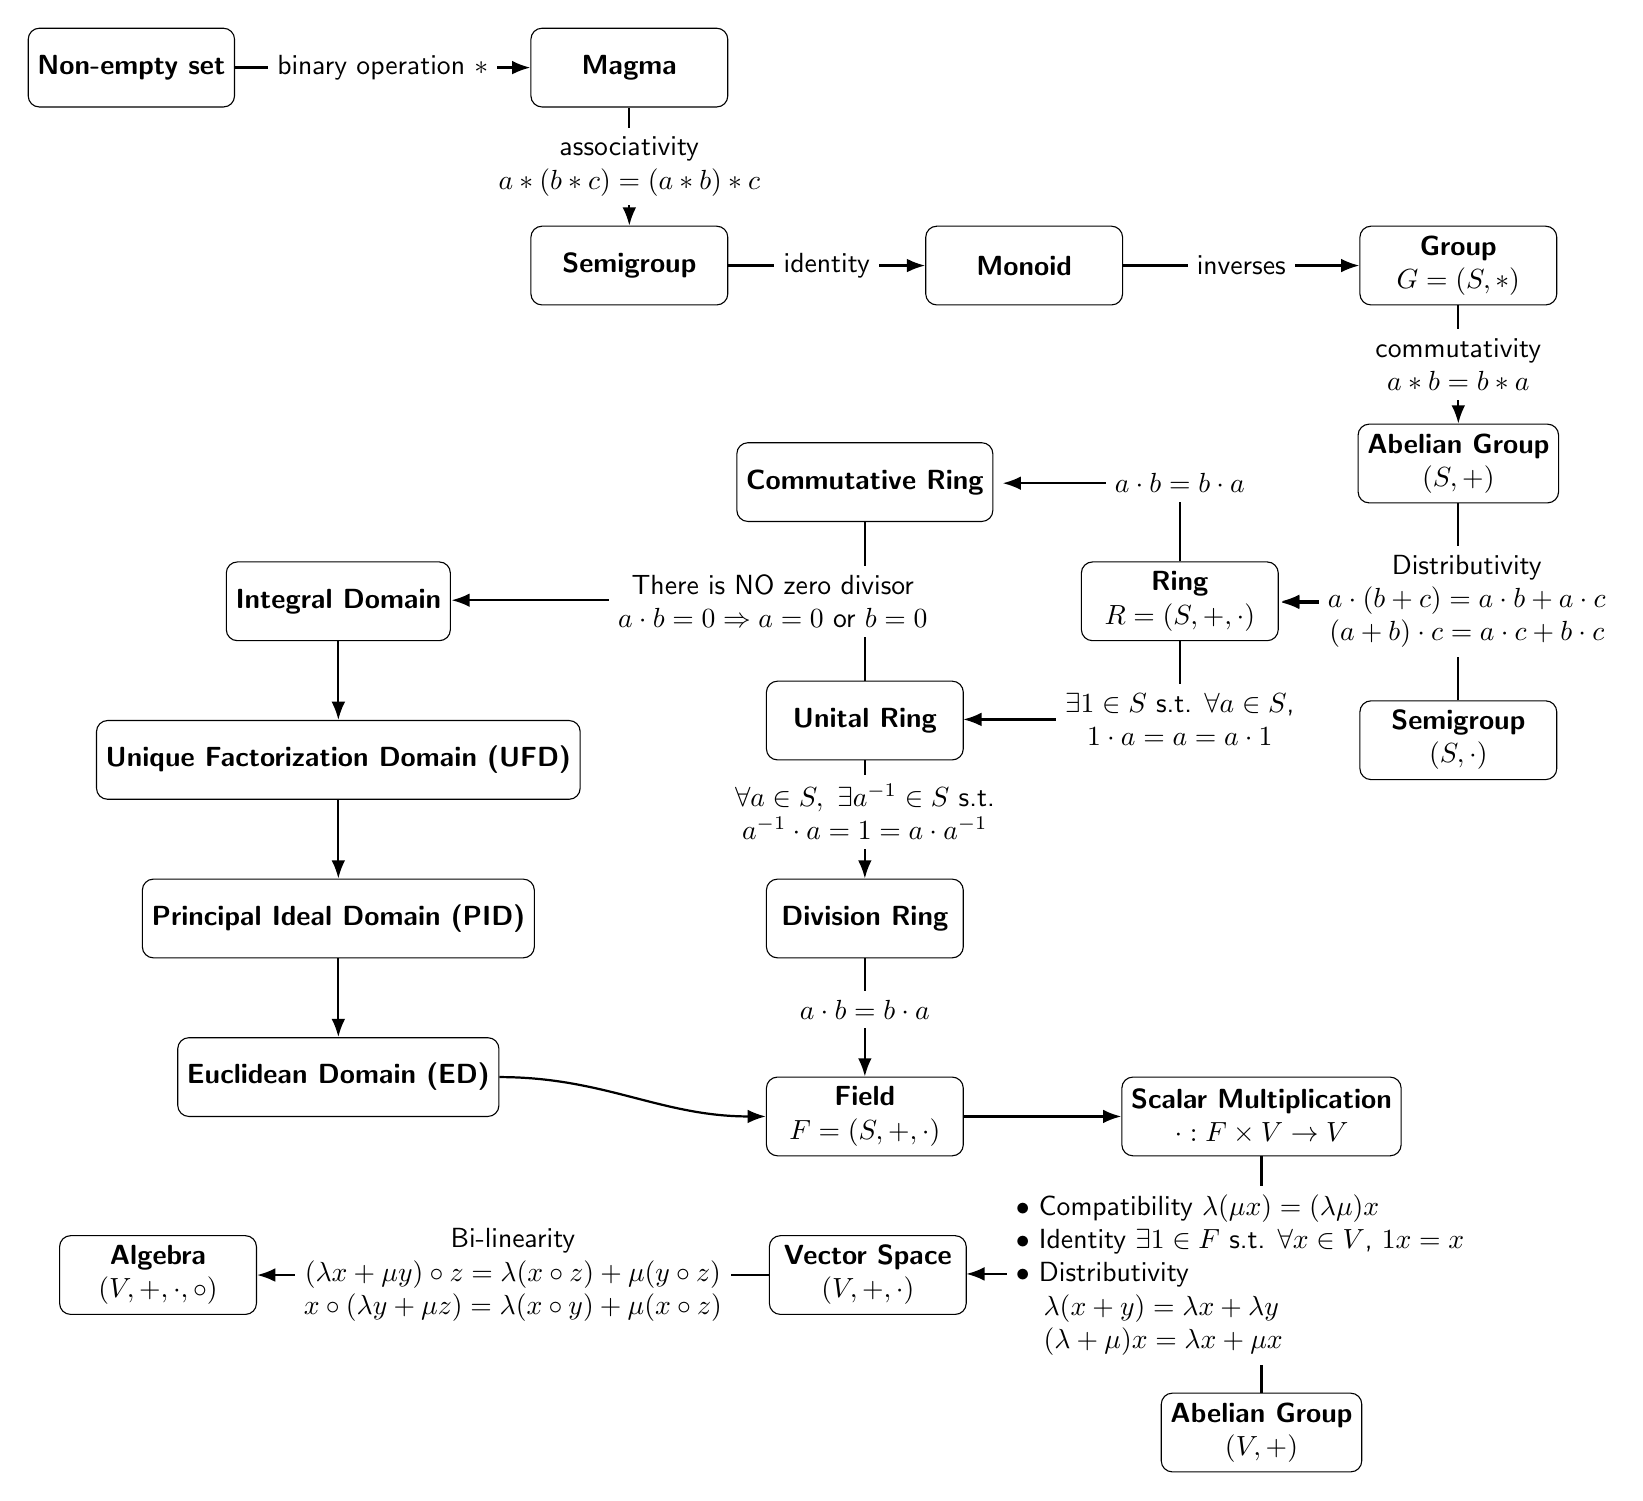
\begin{tikzpicture}[
	node distance=2.5cm,
	every node/.style={font=\sffamily},
	block/.style={
		rectangle, draw, rounded corners,
		minimum width=2.5cm, minimum height=1cm, align=center
	},
	arrow/.style={-Latex, thick}
	]
	
	% Nodes
	\node[block] (set) {\bfseries Non-empty set};
	\node[block, right=3.75cm of set] (magma) {\bfseries Magma};
	\node[block, below=1.5cm of magma] (semigroup) {\bfseries Semigroup};
	\node[block, right=of semigroup] (monoid) {\bfseries Monoid};
	\node[block, right=3cm of monoid] (group) {\bfseries Group\\ $G=(S,*)$};
	\node[block, below=1.5cm of group] (abelian) {\bfseries Abelian Group\\ $(S,+)$};
	\node[block, below=2.5cm of abelian] (semi) {\bfseries Semigroup\\ $(S,\cdot)$};
	\node[block, left=1cm of abelian, yshift=-1.75cm] (ring) {\bfseries Ring\\ $R=(S,+,\cdot)$};
	\node[block, below=.5cm of ring, xshift=-4cm] (unital) {\bfseries Unital Ring};
	\node[block, above=.5cm of ring, xshift=-4cm] (commutative-ring) {\bfseries Commutative Ring};
	\node[block, left=8cm of ring] (id) {\bfseries Integral Domain};
	\node[block, below=1cm of id] (ufd) {\bfseries Unique Factorization Domain (UFD)};
	\node[block, below=1cm of ufd] (pid) {\bfseries Principal Ideal Domain (PID)};
	\node[block, below=1cm of pid] (ed) {\bfseries Euclidean Domain (ED)};
	\node[block, below=1.5cm of unital] (division-ring) {\bfseries Division Ring};
	\node[block, below=1.5cm of division-ring] (field) {\bfseries Field\\ $F=(S,+,\cdot)$};
	\node[block, right=2cm of field] (scalar) {\bfseries Scalar Multiplication\\ $\cdot:F\times V\to V$};
	\node[block, below=3cm of scalar] (commutative-group) {\bfseries Abelian Group\\ $(V,+)$};
	\node[block, below=1cm of scalar, xshift=-5cm] (vector) {\bfseries Vector Space\\ $(V,+,\cdot)$};
	\node[block, left=6.5cm of vector] (algebra) {\bfseries Algebra\\ $(V,+,\cdot, \circ)$};
	
	% Arrows with labels
	\draw[arrow] (set) -- node[fill=white, align=center] {binary operation $\ast$} (magma);
	\draw[arrow] (magma) -- node[fill=white, align=center] {associativity\\ $a*(b*c)=(a*b)*c$} (semigroup);
	\draw[arrow] (semigroup) -- node[fill=white, align=center] {identity} (monoid);
	\draw[arrow] (monoid) -- node[fill=white, align=center] {inverses} (group);
	\draw[arrow] (group) -- node[fill=white, align=center] {commutativity\\ $a*b=b*a$} (abelian);
	\draw[arrow] (abelian) -- ++(0,-1.75) -- ++(-2.25,0);
	\draw[arrow] (semi) -- ++(0,1.75) -- ++(-2.25,0);
	\node[right=.5cm of ring, align=center, fill=white] {Distributivity\\ $a\cdot (b+c)=a\cdot b+a\cdot c$\\ $(a+b)\cdot c=a\cdot c+b\cdot c$};
	\draw[arrow] (ring) -- node[fill=white, align=center, yshift=.5cm] {$a\cdot b=b\cdot a$} ++(0,1.5) -- ++(-2.25,0);
	\draw[arrow] (ring) -- node[fill=white, align=center, yshift=-.5cm] {$\exists 1\in S$ s.t. $\forall a\in S$,\\ $1\cdot a=a=a\cdot 1$} ++(0,-1.5) -- ++(-2.75,0);
	\draw[arrow] (commutative-ring) -- ++(0,-1.5) -- ++(-5.25,0);
	\draw[arrow] (unital) -- ++(0,1.5) -- ++(-2.75,0);
	\node[right=2cm of id, align=center, fill=white] {There is NO zero divisor\\ $a\cdot b=0\Rightarrow a=0\ \text{or}\ b=0$};
	\draw[arrow] (id) -- (ufd);
	\draw[arrow] (ufd) -- (pid);
	\draw[arrow] (pid) -- (ed);
	\draw[arrow, out=0, in=180] (ed) to (field);
	\draw[arrow] (unital) -- node[fill=white, align=center, yshift=.1cm] {$\forall a\in S,\ \exists a^{-1}\in S$ s.t.\\ $a^{-1}\cdot a=1=a\cdot a^{-1}$} (division-ring);
	\draw[arrow] (division-ring) --  node[fill=white, align=center, yshift=.1cm] {$a\cdot b=b\cdot a$} (field);
	\draw[arrow] (field) -- (scalar);
	\draw[arrow] (scalar) -- ++(0,-2) -- ++(-3.75,0);
	\draw[arrow] (commutative-group) -- ++(0,2) -- ++(-2,0);
	\node[right=.5cm of vector, align=left, fill=white] {$\bullet$ Compatibility\ $\lambda(\mu x)=(\lambda\mu)x$\\ $\bullet$ Identity\ $\exists 1\in F$ s.t. $\forall x\in V$, $1x=x$\\ $\bullet$ Distributivity\\
	\hspace{10pt}$\lambda(x+y)=\lambda x+\lambda y$\\ \hspace{10pt}$(\lambda+\mu)x=\lambda x+\mu x$};
	\draw[arrow] (vector) -- node[fill=white, align=center] {Bi-linearity\\ $(\lambda x+\mu y)\circ z=\lambda(x\circ z)+\mu(y\circ z)$\\ $x\circ(\lambda y+\mu z)=\lambda(x\circ y)+\mu(x\circ z)$} (algebra);
\end{tikzpicture}
\end{document}